

\documentclass[fleqn, 12pt]{article}
\usepackage[T1]{fontenc}
\usepackage{tocloft}
\usepackage[margin=1.1in]{geometry} 
\usepackage{amsmath,amsthm,amssymb,amsfonts, fancyhdr, color, comment, graphicx, environ}
\usepackage{xcolor}
\usepackage{mdframed}
\usepackage[shortlabels]{enumitem}
\usepackage{indentfirst}
\usepackage{hyperref}
\usepackage[serbian]{babel}
\renewcommand{\footrulewidth}{1 pt}
\hypersetup{
    colorlinks=true,
    linkcolor=blue,
    filecolor=magenta,      
    urlcolor=blue,
}


\pagestyle{fancy}



\newenvironment{problem}[2][Problem]
    { \begin{mdframed}[backgroundcolor=gray!20] \textbf{#1 #2} \\}
    {  \end{mdframed}}


\newenvironment{solution}{\textbf{Solution}}


\lhead{Pavle Veličković}
\rhead{Računarstvo i društvo} 
\chead{\textbf{}}
\lfoot{Prof. Sana Stojanović Đurđević}
\rfoot{Matematički fakultet, Beograd}

\renewcommand{\contentsname}{Sadržaj}
\begin{document}
\title{\Large Kurs: Računarstvo i društvo  \\[0.5cm]
        \bf\Large OSINT - Lupa u moru}
\author{\large Autor: \bf Mitar Avramović\\ \ \\}
\date{\large Datum: \today}

\makeatletter
    \begin{titlepage}
        \begin{center}
	    {\ \\ \ \\}
        \vbox{}\vspace{5cm}
            {\@title }\\[3cm] 
            {\@author}
            {\large Predmetni profesor: \bf Doc. dr Sana Stojanović Đurđević\\  \ \\}
            {\@date\\}

        \end{center}
    \end{titlepage}
\makeatother


\setcounter{tocdepth}{2}
\tableofcontents

\newpage

\section{Šta su kvantni računari?}

\begin{text}
Kvantni računari su računari koji koriste principe kvantne mehanike. Kvantna mehanika je teorija fizičkog sveta koja nije deterministička, već zasnovana na verovatnoći. Fizički mali sistemi koji se ne ponašaju u skladu sa aproksimacijama jednačina klasične fizike se zovu kvantni sistemi. \cite{G1} Kvantni računari, za razliku od klasičnih, ne koriste bitove za rad, već qubite, i primenjuju fenomene kvatne mehanike u računanju.
\end{text}

\subsection{Razlika između bitova i qubita}

\begin{text}
Kod klasičnih računara, podaci se predstavljaju bitovima, koji mogu postojati u jednom od dva stanja: 0 ili 1. Qubiti se razlikuju od bitova po tome što, pored osnovnih stanja koja se Dirakovom notacijom zapisuju kao \(|0\rangle\) i \(|1\rangle\), mogu biti i u superpoziciji ova dva stanja. Kvantni sitemi mogu postojati u superpoziciji dva ili više stanja, čija se talasna funkcija može opisati kao linearna kombinacija tih stanja. \cite{G1} Kada se u kvantnom sistemu izvrši merenje, kao rezultat se dobije jedno stanje, a ostala stanja se gube. Jedan primer moguće superpozicije qubita je \(|\psi\rangle = a|0\rangle + b|1\rangle\) gde su \(a\) i \(b\) kompleksni brojevi, a \(|a|^2\) i \(|b|^2\) verovatnoće da kada izmerimo kvantni sitem kao rezultat dobijemo \(|0\rangle\) ili \(|1\rangle\). Pri merenju qubita, informacija o koeficijentima (i verovatnoćama) se gubi. \cite{G1} Mogućnost qubita da postoje u više stanja odjednom zbog superpozicije omogućava kvantnim računarima mnogo veću efikasnost u rešavanju određenih problema. Na primer, dok 8 bitova klasičnog računara mogu u jednom trenutku predstavljati samo jedno moguće stanje, 8 qubita mogu biti u superpoziciji 256 različitih stanja. Izračunavanja sa qubitima vrše se nad svim stanjima u superpoziciji u isto vreme. Na primer: \(2 + (|0\rangle + |1\rangle + |4\rangle + |5\rangle) = |2\rangle + |3\rangle + |6\rangle + |7\rangle\), dobija se superpozicija rezultata. U sistemima sa više qubita, qubiti mogu biti upleteni, što znači da merenje stanja jednog qubita može uticati na stanja qubita upletenih sa tim qubitom. Matematički, ovo znači da se talasna funkcija sistema qubita ne može zapisati kao proizvod talasnih funkcija pojedinačnih qubita. \cite{G1}
\end{text}

\begin{figure}[h!]
    \centering
    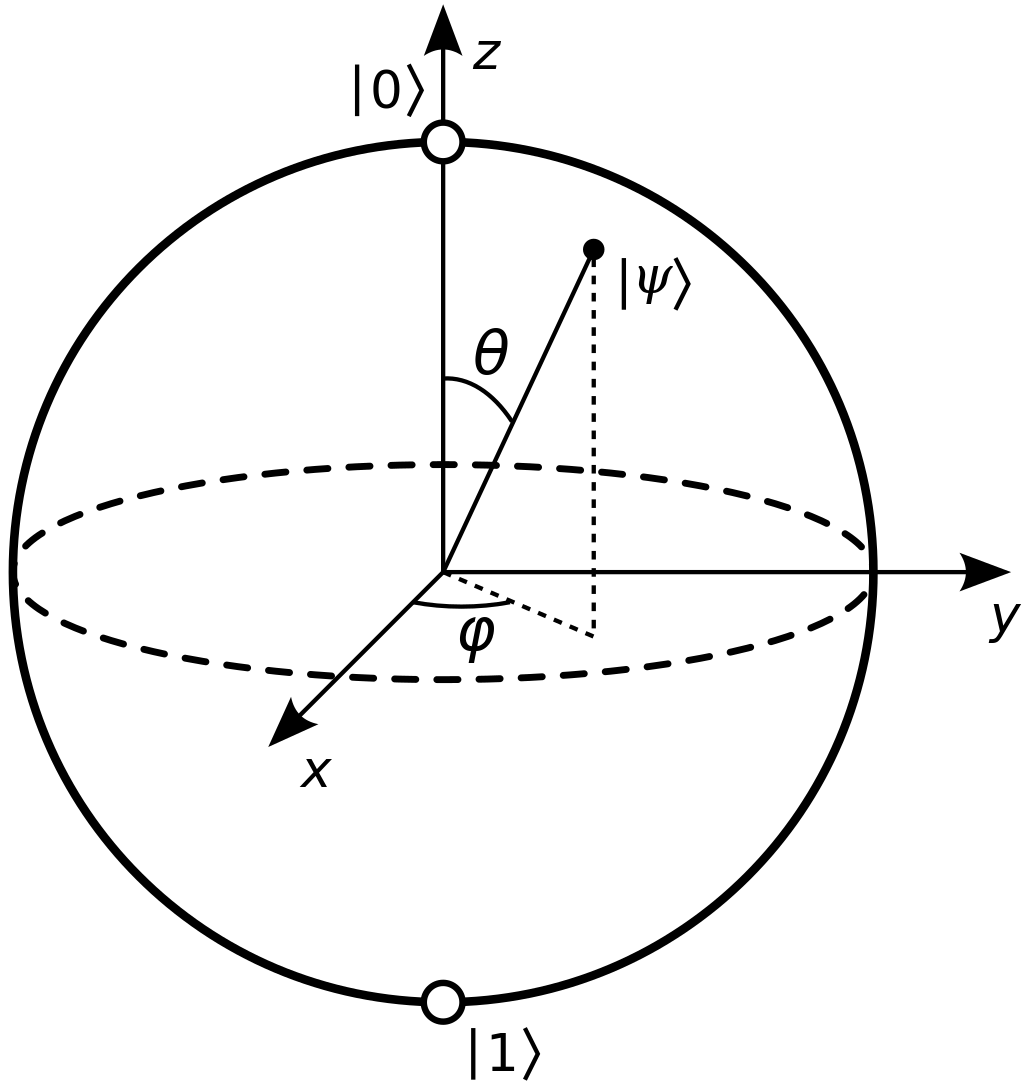
\includegraphics[width=0.35\textwidth]{Bloch_sphere.svg}
    \caption{Blohova sfera, vizuelna reprezentacija qubita}
\end{figure}

\newpage

\subsection{Qubit tehnologije}

\begin{text}
Da bi se kvantno računanje primenilo, potrebno je konstruisati fizičke sisteme u kojima je moguć rad sa qubitima. Konstrukcija i razvoj kvantnih računara se oslanja na istraživanja qubit tehnologija da bi se pronašle najbolje opcije. Trenutno su najrazvijenije tehnologije superprovodničkih qubita i zarobljenih jonskih qubita, ali postoje i druge opcije. \cite{G1}

Zarobljeni jonski qubiti su prvobitno iskorišćeni 1995. godine za demonstraciju kvantnog logičkog kola. \cite{G1} Sistem zarobljenih jonskih qubita je zasnovan na jonima zarobljenim na specifičnom mestu uz pomoć elektromagnetnih polja, preciznim laserima koji mogu da menjaju njihova kvantna stanja, laserima koji hlade jone i omogućavaju merenje njihovih kvantnih stanja i detektore fotona koji vrše merenje kvantnih stanja zarobljenih jona. \cite{G1} Pošto su sami joni qubiti u ovim sistemima, qubiti ne podležu defektima u proizvodnji. \cite{G1}

Superprovodnički qubiti se zasnivaju na superprovodnicima ohlađenim do temperatura blizu apsolutne nule. Kada se ohlade, superprovodnička elektronska kola koja predstavljaju superprovodnilčke qubite mogu imati kvantizovane energetske nivoe, pa se nazivaju i "veštački atomi", a osnovno i prvo pobuđeno stanje takvog kvantnog sistema se koriste kao dva stanja za qubit. \cite{G1}

Osim ovih opcija se mogu koristiti fotoni, neutralni atomi, poluprovodnički qubiti i topološki qubiti. \cite{G1}
\end{text}

\begin{figure}[h!]
  \centering
  \begin{minipage}[b]{0.4\textwidth}
    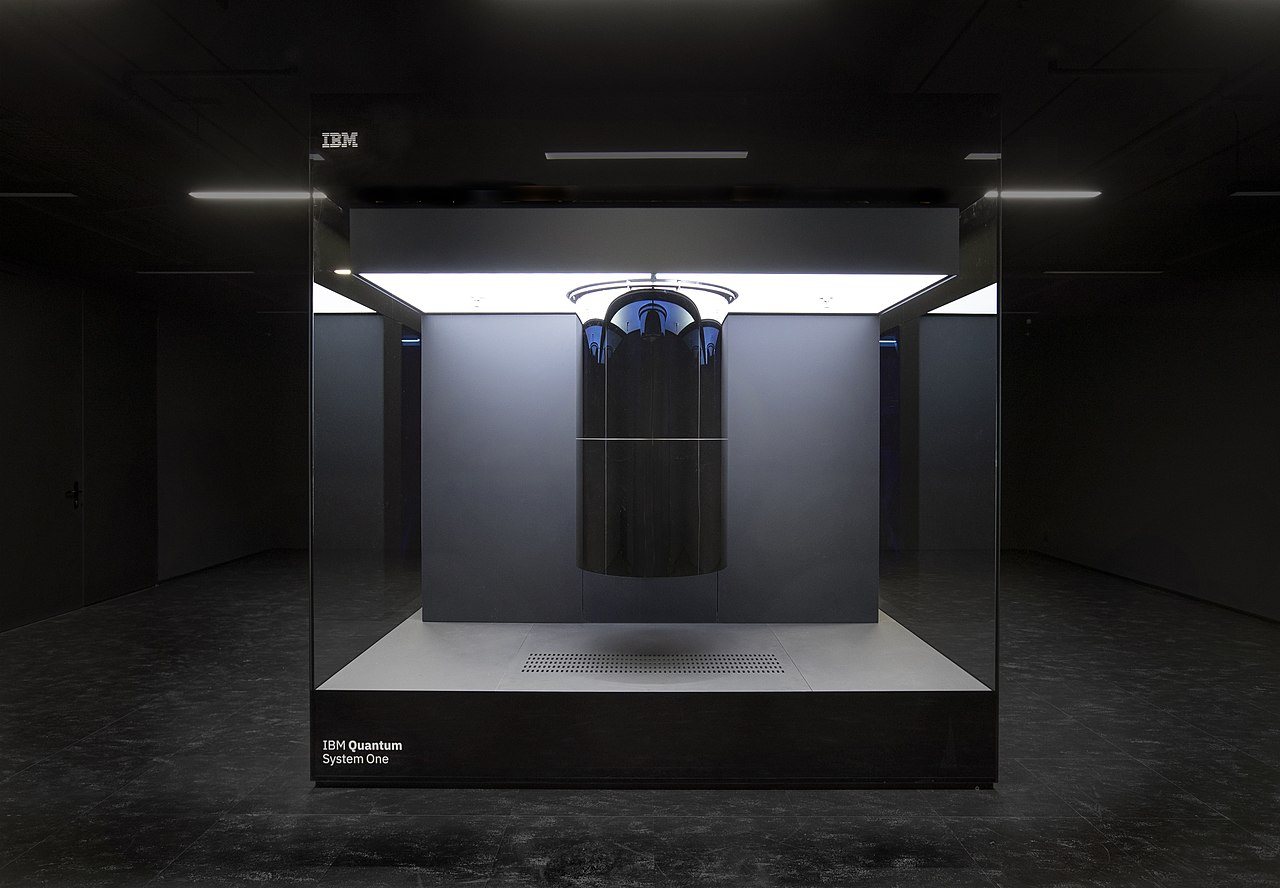
\includegraphics[width=\textwidth]{IBM_Q_system_(Fraunhofer_2).jpg}
    \caption{IBM-ov Quantum System One kvantni računar sa 20 superprovodnička qubita}
  \end{minipage}
  \hfill
  \begin{minipage}[b]{0.4\textwidth}
    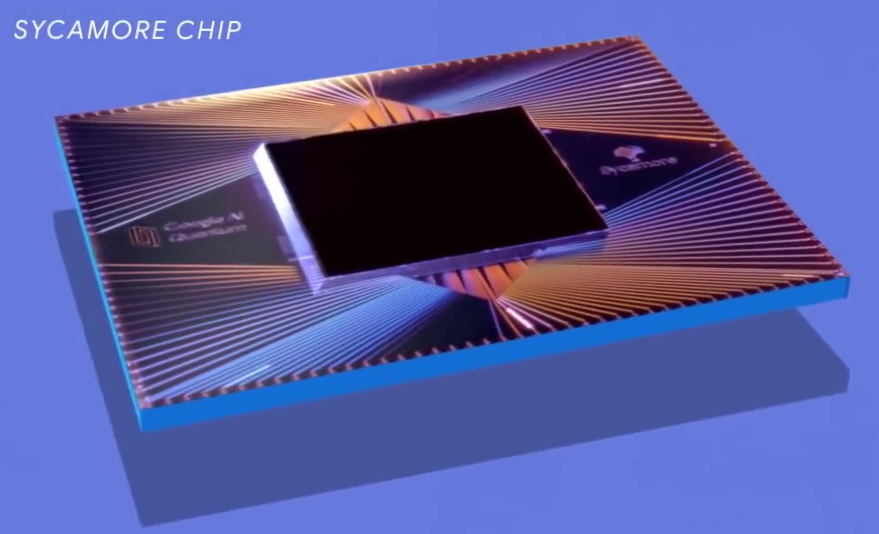
\includegraphics[width=\textwidth]{Google_Sycamore_Chip_002.png}
    \caption{Google-ov Sycamore superprovodnički kvantni procesor sa 53 qubita}
  \end{minipage}
\end{figure}

\newpage

\section{Dobre strane razvoja kvantnih računara}

\begin{text}
Razvoj upotrebljivih kvantnih računara bi mogao značajno da poboljša istraživanja i rešavanje problema u mnogim oblastima. Zbog toga kako kvantni računari funkcionišu i šta sve mogu da postignu što klasični računari ne mogu, mogu se razvijati kvantni algoritmi koji bi određene probleme mogli da rešavaju mnogo brže od klasičnih računara, što bi značajno ubrzalo rešavanje važnih problema.
\\\\

Neke oblasti u kojima bi mogli biti primenjeni kvantni algoritmi su fizika kondenzovane materije, kvantna hemija, nuklearna fizika i fizika čestica, kombinatorijalna optimizacija, neprekidna optimizacija, kriptoanaliza, rešavanje diferencijalnih jednačina, finansije i mašinsko učenje. \cite{G2}

Jedan primer kvantnog algoritma je Groverov algoritam pretrage, koji je jedan od izvora kvantnog ubrzanja. Groverov algoritam nalazi ulazne vrednosti za funkciju koje daju određene povratne vrednosti. \cite{G1} Koristi se za nalaženje minimuma funkcija u problemima kombinatorne (diskretne) optimizacije, jer je mnoge takve probleme moguće svesti na problem pretrage. Neki od problema čije rešavanje Groverov algoritam može da ubrza su k-bojenje, problem trgovačkog putnika, najkraći put između dva čvora u grafu i SAT. \cite{G2}

U velikom broju naučnih polja, kvantne simulacije bi bile mnogo preciznije od simulacija koje mogu da se postignu na klasičnim računarima i veruje se da bi kvantni računari poboljšali razumevanje fizičkih modela. 
\\\\

Da bi kvantni algoritmi stvarno bili bolji od klasičnih, potrebno je iskoristiti kvantne fenomene da bi se postiglo kvantno ubrzanje. Izvor kvantne prednosti su kvantne algoritamske primitive, koje uglavnom nisu rešenje nijednog problema same za sebe, ali se kvantni algoritmi mogu posmatrati kao kompozicija kvantnih algoritamskih primitiva. \cite{G2}

Neke kvantne algoritamske primitive su kvantna linearna algebra, Hamiltonova simulacija, kvantna Furijeova transformacija, kvantna procena faza, amplifikacija i procena amplituda, Gibsovo uzorkovanje, kvantni adijabatski algoritam, kvantni rešavači linearnih sistema jednačina i kvantna procena gradijenata funkcija.
\\\\

Ova poboljšanja sa sobom nose izazov da se ne mogu jednostavno upotrebiti postojeći algoritmi za rešavanje problema kvantnim računarima jer se neće postići ubrzanje. Kvantni računari nisu potpuna zamena klasičnih računara jer se ne mogu upotrebiti za sve svrhe za koje koristimo klasične računare.
\\\\

U svim poznatim realizacijama kvantnih sistema sa fizičkim qubitima, greške se javljaju previše često da bi se većina poznatih kvantnih algoritama zapravo primenilo. \cite{G2} Da bi se minimizovao broj grešaka, razvijaju se pristupi ispravljanja grešaka i ublažavanja grešaka. \cite{G1}
\end{text}

\newpage

\subsection{Kvantna nadmoć}

\begin{text}
Kvantna nadmoć je trenutak u razvoju kvantnih računara kada se pokaže da kvantni računari mogu da izvrše kvantno izračunavanje koje je za klasične računare teško. Kvantna nadmoć bi dokazala da su kvantni računari stvarno korisni. \cite{G1}

Da bi se ovako nešto postiglo, potrebno je konstruisati dovoljno veliki kvantni računar i naći problem koji on može da reši, a klasični računari ne mogu u razumnom vremenu. \cite{G1}

Velike tehnološke kompanije se trude da razviju kvantne računare koji će postići kvantnu nadmoć, ali još uvek nije poznato da li će i kada zaživeti praksa korišćenja kvantnih računara.
\end{text}

\newpage

\section{Loše strane razvoja kvantnih računara}

\begin{text}
Razvoj kvantnih računara ne nosi sa sobom samo dobre ishode. Sam proces razvoja kvantnih računara je skup i nije poznato da li će upotreba kvantnih računara zaživeti i da li će se istraživanja u polju kvantnih računara isplatiti.

Iako kvantni računari u određenim poljima i za određene probleme predstavljaju veliki napredak, za većinu slučajeva u kojima danas upotrebljavamo klasične računare, kvantni računari neće biti primenjivi. To je ili zato što ne predstavljaju nikakav napredak u odnosu na klasične računare, ili zato što zbog prirode qubita, njihovoj sklonosti greškama i njihovoj osetljivosti na okolinu, kvantni računari jednostavno nisu primenjivi u nekim situacijama.

Međutim, postoji mnogo veći problem koji kvantni računari mogu da prouzrokuju, a tiče se kriptografije i bezbednosti osetljivih podataka. Kvantni računari, zbog svoje potencijalno velike efikasnosti u određenim izračunavanjima, prete da razbiju svu enkripciju koja se danas upotrebljava.
\end{text}

\subsection{Razbijanje kriptografije Šorovim algoritmom}

\begin{text}
Današnja kriptografija se zasniva uglavnom na "one-way" funkcijama koje se mogu lako izračunati ali se ne mogu lako invertovati, kao što su hash i trapdoor funkcije. \cite{G5} 

Kriptografije zasnovane na javnim ključevima su najčešće korišćene za enkriptovanje lozinki, privatnih poruka i ostalih osetljivih podataka. Jedan kriptosistem javnih ključeva koji je u širokoj upotrebi je RSA sistem. RSA sistem ima javni enkripcioni ključ \((e,n)\) i privatni dekripcioni ključ \((d,n)\), gde je broj \(n\) proizvod dva velika slučajna prosta broja, \(n = p * q\), \(d\) je uzajamno prost sa proizvodom \((p - 1) * (q - 1)\), a \(e\) je multiplikativni inverz broja \(d\) modulo \((p - 1) * (q - 1)\). Iako je broj \(n\) javno dostupan, \(p\) i \(q\) se ne mogu jednostavno izračunati zato što je faktorizacija velikih brojeva težak problem za klasične računare. \cite{G3}
\\\\

Kvantni računari, uz pomoć Šorovog algoritma, mogu veoma brzo i efikasno da faktorizuju velike brojeve. \cite{G4}

Za bilo koji ceo broj \(n\) i ceo broj \(x\) za koji važi \(1 < x < n\), važi da postoji broj \(r\) takav da je \(x^r \equiv 1\, ( \bmod\, n)\). Prvo izaberemo slučajan broj \(x\) za koji važi \(1 < x < n\). Ako \(x\) i \(n\) nisu uzajamno prosti, njihov najveći zajednički delilac je jedan od faktora broja \(n\), pa možemo naći i drugi. Ako su uzajamno prosti, algoritam se nastavlja.
Pošto  \(x^r \equiv 1\, ( \bmod\, n)\), onda \(x^r - 1 \equiv 0\, ( \bmod\, n)\), što znači da \((x^{r/2} - 1)*(x^{r/2} + 1) \equiv 0\, ( \bmod\, n)\). Ako je \(r\) neparan, ponovo slučajno biramo \(x\) i računamo ispočetka. Ako je \(r\) paran, onda tražimo najveći zajednički delilac za \((x^{r/2} - 1)\) i \(n\), koji možemo naći Euklidovim algoritmom i obeležimo ga sa \(p\).
Kada nađemo taj faktor broja \(n\), drugi faktor nalazimo kao \(q = n/p\). \cite{G4}

\end{text}

\newpage

\begin{text}
Na primeru možemo uočiti da se svi moduli periodično ponavljaju, svakih r puta. Ako je \(p = 5, q = 7, n = 35, x = 4\), imamo \(4^1 \equiv 4\, ( \bmod\, 35)\), \(4^2 \equiv 16\, ( \bmod\, 35)\), \(4^3 \equiv 29\, ( \bmod\, 35)\), \(4^4 \equiv 11\, ( \bmod\, 35)\), \(4^5 \equiv 9\, ( \bmod\, 35)\), \(4^6 \equiv 1\, ( \bmod\, 35)\), dakle \(r = 6\). Možemo proveriti, na primer, da je 
\(4^3 \equiv 4^9 \equiv 4^{15} \equiv \,... \, \equiv 29\, ( \bmod\, 35)\). Uz pomoć kvantne Furijeove transformacije, pošto se rezultat modulo \(n\) ponavlja na svakih \(r\) broja, i pošto znamo da je \(x^0 \equiv 1\, ( \bmod\, n)\), dovoljno je da se izmeri bilo koji modulo iz nekog qubita i da se na preostaloj superpoziciji stanja, u ovom slučaju \(|3\rangle|29\rangle + |9\rangle|29\rangle + |15\rangle|29\rangle + ...\), primeni kvantna Furijeova transformacija, čiji će rezultat biti \(|1/6\rangle\), u opštem slučaju \(|1/p\rangle\), pa frekvenciju ponavljanja modula možemo odrediti iz rezultata kao \(1/rezultat\), u ovom slučaju \(r = 6\). Ovaj proces značajno ubrzava faktorizaciju, koja bi za velike brojeve bila neizvodljiva na klasičnom računaru. \cite{G4}
\\\\

U praksi je za ovako nešto trenutno potreban veliki broj qubita i veoma precizna kontrola nad kvantnim sistemom, ali se vremenom qubit tehnologije poboljšavaju i čini se da je broj qubita potreban za razbijanje enkripcije sve manji i manji, a broj qubita u postojećim kvantnim računarima se povećava. U trenutku kada neki kvantni računar bude imao dovoljan broj qubita dobrog kvaliteta i način da se njima precizno upravlja, problem faktorizacije velikih brojeva će biti lako rešiv i postojeća enkripcija više neće biti bezbedna, jer će se od javnih ključeva lako dolaziti do privatnih, što sa klasičnim računarima nije moguće.
\end{text}

\subsection{Post-kvantna kriptografija}

\begin{text}
Zbog opasnosti po kriptografiju koje predstavljaju kvantni računari, već neko vreme se traže kriptosistemi koji će biti otporni na napade i od strane klasičnih i od strane kvantnih računara. Za sada su identifikovana četiri algoritama za enkripciju koji će moći da budu deo post-kvantne kriptografije: \cite{G6}
\end{text}

\begin{enumerate}
  \item CRYSTALS-Kyber, algoritam za enkripciju generalno i za uspostavljanje ključeva, zasnovan na rešetkama. \cite{G6}
  \item CRYSTALS-Dilithium, algoritam za digitalne potpise (digital signature), zasnovan na rešetkama. \cite{G6}
  \item Falcon, algoritam za digitalne potpise, zasnovan na rešetkama. \cite{G6}
  \item Sphincs+, algoritam za digitalne potpise, zasnovan na hash funkciji. \cite{G6}
\end{enumerate}

\begin{text}
Rešetke su skup tačaka u n-dimenzionom prostoru takav da je zbir vektora položaja bilo koje dve tačke u rešetki neka tačka koja takođe pripada toj rešetki. Kriptografija rešetki se smatra ključnim kandidatom za post-kvantnu kriptografiju i zasniva se na kompleksnosti problema vezanih za rešetke. \cite{G6}
\end{text}

\newpage

\begin{text}
Problemi na koje se oslanja kriptografija rešetki su problem najkraćeg vektora (SVP, shortest vector problem) i problem najbližeg vektora (CVP, closest vector problem). \cite{G6}
\\\\

Problem najkraćeg vektora je određivanje najkraćeg nenula vektora \(\mathbf{v}\) koji pripada nekoj n-dimenzionoj rešetki \(\Lambda\), tačnije vektora \(\mathbf{v} \in \Lambda\) čija je Euklidska norma \(||\mathbf{v}||\) najmanja. \cite{G6}

Problem najbližeg vektora je, za dati n-dimenzioni vektor \(\mathbf{w}\) koji ne pripada n-dimenzionoj rešetki \(\Lambda\), naći vektor \(\mathbf{v}\) koji pripada toj rešetki koji je najbliži vektoru \(\mathbf{w}\), tačnije za \(\mathbf{w} \notin \Lambda\) naći \(\mathbf{v} \in \Lambda\) za koji je Euklidska norma \(||\mathbf{w} - \mathbf{v}||\) najmanja. \cite{G6}
\\\\

Za probleme SVP i CVP je poznato da su na klasičnim računarima NP-teški. Što se tiče kvantnih računara, za sada nije pronađen nijedan algoritam koji može u polinomskom vremenu da reši bilo koji od ovih problema, ali nije dokazano ni da takav algoritam ne postoji. Najviše se veruje pretpostavkama da kvantni algoritmi za rešavanje ovih problema u polinomskom vremenu ne postoje. \cite{G6}
\end{text}

\newpage

\section{Etika i kvantni računari}

\begin{text}
Kao i svaka nova tehnologija, kvantni računari sa sobom nose veliki potencijal. Nažalost, postoje ljudi, organizacije i vlade koje žele da potencijal kvantnih računara zloupotrebe.
\\\\

U vezi sa kvantnim računarima postoje etičke dileme zbog mogućnosti zloupotrebe, jer će kvantni računari, ako se uspešno razviju, pored svega dobrog čemu će moći da doprinesu, na primer rešavanju važnih problema koji su za klasične računare izuzetno teški, takoge moći da doprinesu lošim stvarima kao što su urušavanje bezbednosti podataka.
\\\\

Kvantne simulacije, ako se dovoljno razviju, moći će da se upotrebe za mnogo dobrih stvari i za napredak u svim poljima, ali će isto tako moći da se zloupotrebe. Sa dobre strane, moći će da doprinesu napretku u medicini, genetici, proučavanju prirodnih pojava, astronomiji, itd., ali sa loše strane, moći će da se upotrebe za pravljenje novih oružja.
\\\\

Zbog svega ovog je problematična činjenica da će kvantni računari možda u bliskoj budućnosti biti mnogo dostupniji i mnogo moćniji, što će omogućiti da padnu u pogrešne ruke i budu zloupotrebljeni.
\end{text}

\newpage

\section{Privatnost na internetu i bezbednost interneta u eri kvantnih računara}

\begin{text}
Kvantni računari predstavljaju ozbiljnu pretnju privatnosti na internetu, jednostavno zbog svojih mogućnosti da vrše određena izračunavanja mnogo brže od klasičnih računara.
\\\\

Sa razvojem kvantnih računara razvijaju se i algoritmi kao što je Šorov algoritam, koji mogu u potpunosti da probiju enkripciju koja se danas koristi za zaštitu lozinki, privatnih poruka i ostalih osetljivih podataka. Ovo je neizbežno sa razvojem kvantnih računara i neophodno je preći na kriptografiju koja se ne može probiti kvantnim algoritmima.
\\\\

Međutim, već se praktikuje nešto što se zove "Harvest Now Decrypt Later", gde vlade država, hakeri i drugi potencijalno maliciozni pojedinci i organizacije prikupljaju enkriptovane podatke u nadi da će u skorijoj budućnosti moći da ih dekriptuju pomoću kvantnih računara i kvantnih algoritama.
\\\\

Narušavanje privatnosti može i negativno uticati na bezbenost ljudi na internetu, u slučaju da budu targetirani od strane nekoga sa malicioznim namerama.
\\\\

Ako kvantni računari budu široko rasprostranjeni i lako dostupni, što se danas ne čini verovatnim, ali nije nemoguće u budućnosti, to otvara vrata mogućnosti da ih veliki broj ljudi zloupotrebi da ugrozi tuđu privatnost, a potencijalno i bezbednost, na primer u slučaju da su osetljivi podaci podeljeni u privatnim porukama koje budu dekriptovane.
\\\\

Ostaje pitanje da li će biti novih zakona i regulacija širom sveta što se tiče kvantnih računara da se ne bi zloupotrebili za ugrožavanje privatnosti i bezbednosti.
\end{text}

\newpage

\section{Zaključak}

\begin{text}
Kvantni računari su još uvek nova tehnologija koja nije u potpunosti ni razvijena, i do danas nisu postigli ništa revolucionarno. Ipak, u budućnosti bi mogli da dodju dotle da su mnogo moćniji od klasičnih računara, pa čak i da zažive u širokoj upotrebi i budu lako dostupni. Potrebno je spremiti se za budućnost u kojoj kvantni računari mogu da probiju sve jednostavnije metode zaštite podataka, pa čak i da budu zloupotrebljeni u druge svrhe. Sa druge strane, kvantni računari bi mogli da doprinesu poboljšanju kvaliteta ljudskih života ako budu upotrebljeni na taj način. 

Danas kvantni računari imaju mali broj qubita, tehnologije nisu razvijene u dovoljnoj meri da kvantni računari stvarno bilo šta značajno promene i kvantni algoritmi koji su razvijeni nisu upotrebljeni u praksi za postizanje bilo kakvih revolucionarnih promena, ali bi sve to moglo da se naglo promeni u bliskoj budućnosti, što bi značajno promenilo dosta doga, na bolje ili na gore. Predviđanja su različita, a postoji i verovanje da kvantni računari nikada neće moći da se razviju dovoljno za bilo kakvu značajnu upotrebu.
\end{text}

\newpage
{
\raggedright
\renewcommand{\refname}{Reference}
\begin{thebibliography}{9}
    \bibitem{G1} Quantum Computing Progress and Prospects (2019), National Academies of Sciences, Engineering, and Medicine; Division on Engineering and Physical Sciences; Computer Science and Telecommunications Board; Intelligence Community Studies Board; Committee on Technical Assessment of the Feasibility and Implications of Quantum Computing; Emily Grumbling and Mark Horowitz, Editors \href{https://nap.nationalacademies.org/catalog/25196/quantum-computing-progress-and-prospects}{nap.nationalacademies.org}
    
    \bibitem{G2} Quantum algorithms: A survey of applications and end-to-end complexities (2023), Alexander M. Dalzell, Sam McArdle, Mario Berta, Przemyslaw Bienias, Chi-Fang Chen, András Gilyén, Connor T. Hann, Michael J. Kastoryano, Emil T. Khabiboulline, Aleksander Kubica, Grant Salton, Samson Wang, Fernando G. S. L. Brandão \href{https://arxiv.org/abs/2310.03011}{arxiv.org}
    
    \bibitem{G3} A Method for Obtaining Digital Signatures and Public-Key Cryptosystems (1978), R.L. Rivest, A. Shamir, L. Adleman \href{http://people.csail.mit.edu/rivest/Rsapaper.pdf}{people.csail.mit.edu}
    
    \bibitem{G4} Polynomial-Time Algorithms for Prime Factorization and Discrete Logarithms on a Quantum Computer (1996), Peter W. Shor \href{https://arxiv.org/abs/quant-ph/9508027}{arxiv.org}
    
    \bibitem{G5} Post Quantum Cryptography and its Comparison with Classical Cryptography (2024), Tanmay Tripathi, Abhinav Awasthi, Shaurya Pratap Singh, Atul Chaturvedi \href{https://arxiv.org/abs/2403.19299}{arxiv.org}
    
    \bibitem{G6} The Mathematical Foundation of Post-Quantum Cryptography (2024), Chuanming Zong \href{https://arxiv.org/abs/2404.19186}{arxiv.org}
\end{thebibliography}
}
\end{document}